\section{Résultats}

Comme mentionné en introduction, nous avons testé trois méthodes de vectorisation : TF-IDF, doc2vec et BERT
Nous avons utilisé ces vecteurs pour entraîner et comparer 4 modèles différents : Régression logistique, SVM, Random Forest et Perceptron.


\begin{table}[h]
    \centering
    \begin{tabular}{|l|l|l|l|l|}
        \hline
        & Clf & RandomForest & SVM & Perceptron & LR \\
        \hline
        Anglais & 0.37 & \textbf{0.47} & 0.41 & 0.46 \\
        \hline
        Français & 0.34 & \textbf{0.45} & 0.42 & 0.44 \\
        \hline
        Italien & 0.33 & \textbf{0.43} & 0.40 & 0.43 \\
        \hline
    \end{tabular}
    \caption{F-mesure des classifieurs par langue avec vectorisation \texttt{TF-IDF}}
    \label{tab:comparaison_vecteurs}
\end{table}

\begin{table}[h]
    \centering
    \begin{tabular}{|l|l|l|l|l|}
        \hline
        & Clf & RandomForest & SVM & Perceptron & LR \\
        \hline
        Anglais & 0.29 & \textbf{0.39} & 0.22 & 0.31 \\
        \hline
        Français & 0.26 & \textbf{0.34} & 0.25 & 0.28 \\
        \hline
        Italien & 0.27 & \textbf{0.33} & 0.22 & 0.28 \\
        \hline
    \end{tabular}
    \caption{F-mesure des classifieurs par langue avec vectorisation \texttt{Doc2Vec}}
    \label{tab:comparaison_vecteurs}
\end{table}

\begin{table}[h]
    \centering
    \begin{tabular}{|l|l|l|l|l|}
        \hline
        & Clf & RandomForest & SVM & Perceptron & LR \\
        \hline
        Anglais & 0.32 & \textbf{0.32} & 0.22 & 0.36 \\
        \hline
        Français & 0.31 & \textbf{0.27} & 0.13 & 0.36 \\
        \hline
        Italien & 0.31 & \textbf{0.26} & 0.15 & 0.36 \\
        \hline
    \end{tabular}
    \caption{F-mesure des classifieurs par langue avec vectorisation \texttt{BERT}}
    \label{tab:comparaison_vecteurs}
\end{table}


\begin{figure}[t]
  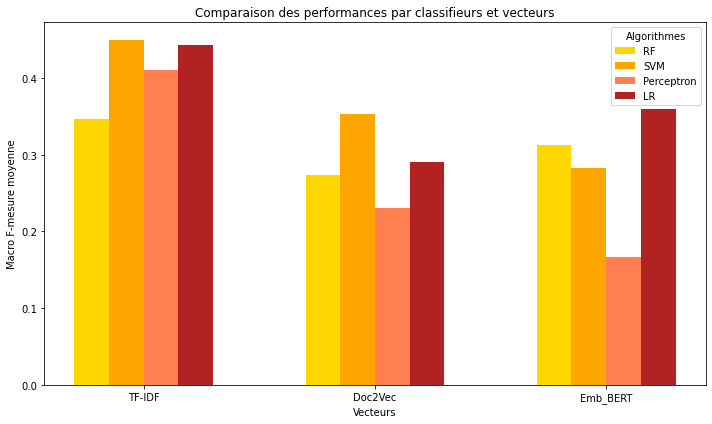
\includegraphics[width=\columnwidth]{"./assets/comparaison_vecteur_clf_barplot.png"}
  \caption{Comparaison des vecteurs et classifieurs.}
  \label{fig:comparaison_vecteur}
\end{figure}